\subsection{ \og Stigmergie \fg{} }

Dans le but de bien dissocier la logique liée à la réflexion de celle qui structure le jeu, nous avons choisi de suivre le paradigme \og Agent et Environnement \fg{}. Notre IA est assimilée à un agent qui évolue dans un environnement qu'il peut observer et modifier.

Toute communication entre agents se fait donc par \og Tableau Noir \fg{}, c'est à dire en laissant des traces dans cet environnement partagé. Cette interaction dite \og Stigmergique\footnote{La stigmergie est une méthode de communication indirecte dans un environnement émergent auto-organisé, où les individus communiquent entre eux en modifiant leur environnement. (Article \og Stigmergie \fg{} de Wikipédia en français, licence CC-BY-SA)} \fg{} est nécessairement asynchrone mais possède l'avantage de ne nécessiter qu'un seul canal de communication par agent. Ce canal, qui relie l'agent à son environnement, est bidirectionnelle : il permet à l'agent de recevoir des stimuli et d'envoyer des impulsions. Dans la suite de ce document, nous parlerons de \og percepts\fg{} et \og actions\fg{}.

\begin{figure}[H] 
\centering
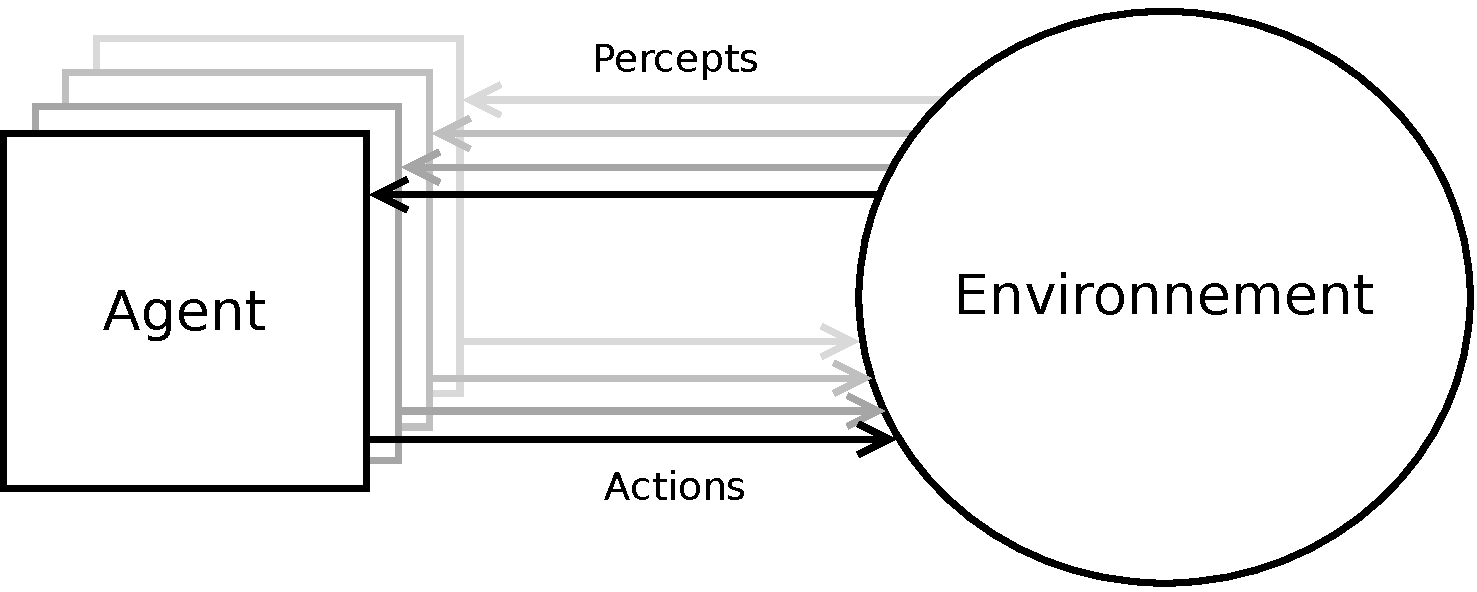
\includegraphics[width=\textwidth]{files/env/agent_env} 
\caption{Modèle \og Agent et Environnement \fg{}} 
\label{agent_env}
\end{figure}

La séparation entre l'agent et son environnement permet de gagner en flexibilité : la communication ne se faisant qu'au travers de l'envoie de messages précis, tout algorithme peut être encapsulé avec une interface simple pour en faire un agent.

L'agent peut donc être un humain ou une machine. Une machine pouvant exécuter notre modèle aussi bien qu'une intelligence artificielle tiers. 

Ainsi, nous disposons d'une abstraction du fonctionnement interne de chaque agent, ce qui permet :
\begin{itemize}
\item d'une part de faire jouer notre agent contre un autre agent basé sur une stratégie connue, facilitant ainsi l'évaluation de notre modèle,
\item d'autre part de tester les développements qui concernent l'environnement avant même que notre IA ne soit fonctionnelle en faisant jouer des agents naïfs entre eux. Cette méthode permet d'isoler pleinement le développement de la plateforme de tests de celui de l'IA.
\end{itemize}

\subsection{ Agent \og Arbitre \fg{} }

Comme indiqué dans la section~\ref{section:domaine_application_le_jeu_de_plateau} (page~\pageref{section:domaine_application_le_jeu_de_plateau}) l'environnement est un jeu de plateau. Il s'agit d'une grille dont les cases peuvent contenir un pion ou être vides.

L'environnement doit aussi être capable de déterminer le prochain joueur qui doit prendre la main ainsi que toute autre information qui ne peut pas être déterminée via l'état du plateau. Il doit également pouvoir juger de la légalité des coups proposés par un agent, et par le même biais savoir comment initialiser le plateau lors d'une nouvelle partie.

Il se décompose donc en trois modules :
\begin{itemize}
\item un plateau,
\item une liste de règles,
\item et un processeur qui les manipules.
\end{itemize}

Plutôt que de briser la métaphore du \og Tableau Noir \fg{} en parlant d'\emph{environnement-agent}, nous avons fait le choix de voir ce processeur comme un agent tiers : une sorte d'arbitre neutre. C'est un agent purement réactif qui maintient l'état du jeu en exécutant les coups qui lui sont envoyés par les agents joueurs dans la mesure du légale. Il doit veiller à notifier le résultat des actions effectuées et envoyer l'état du plateau en cas de demande.

\begin{figure}[H] 
\centering
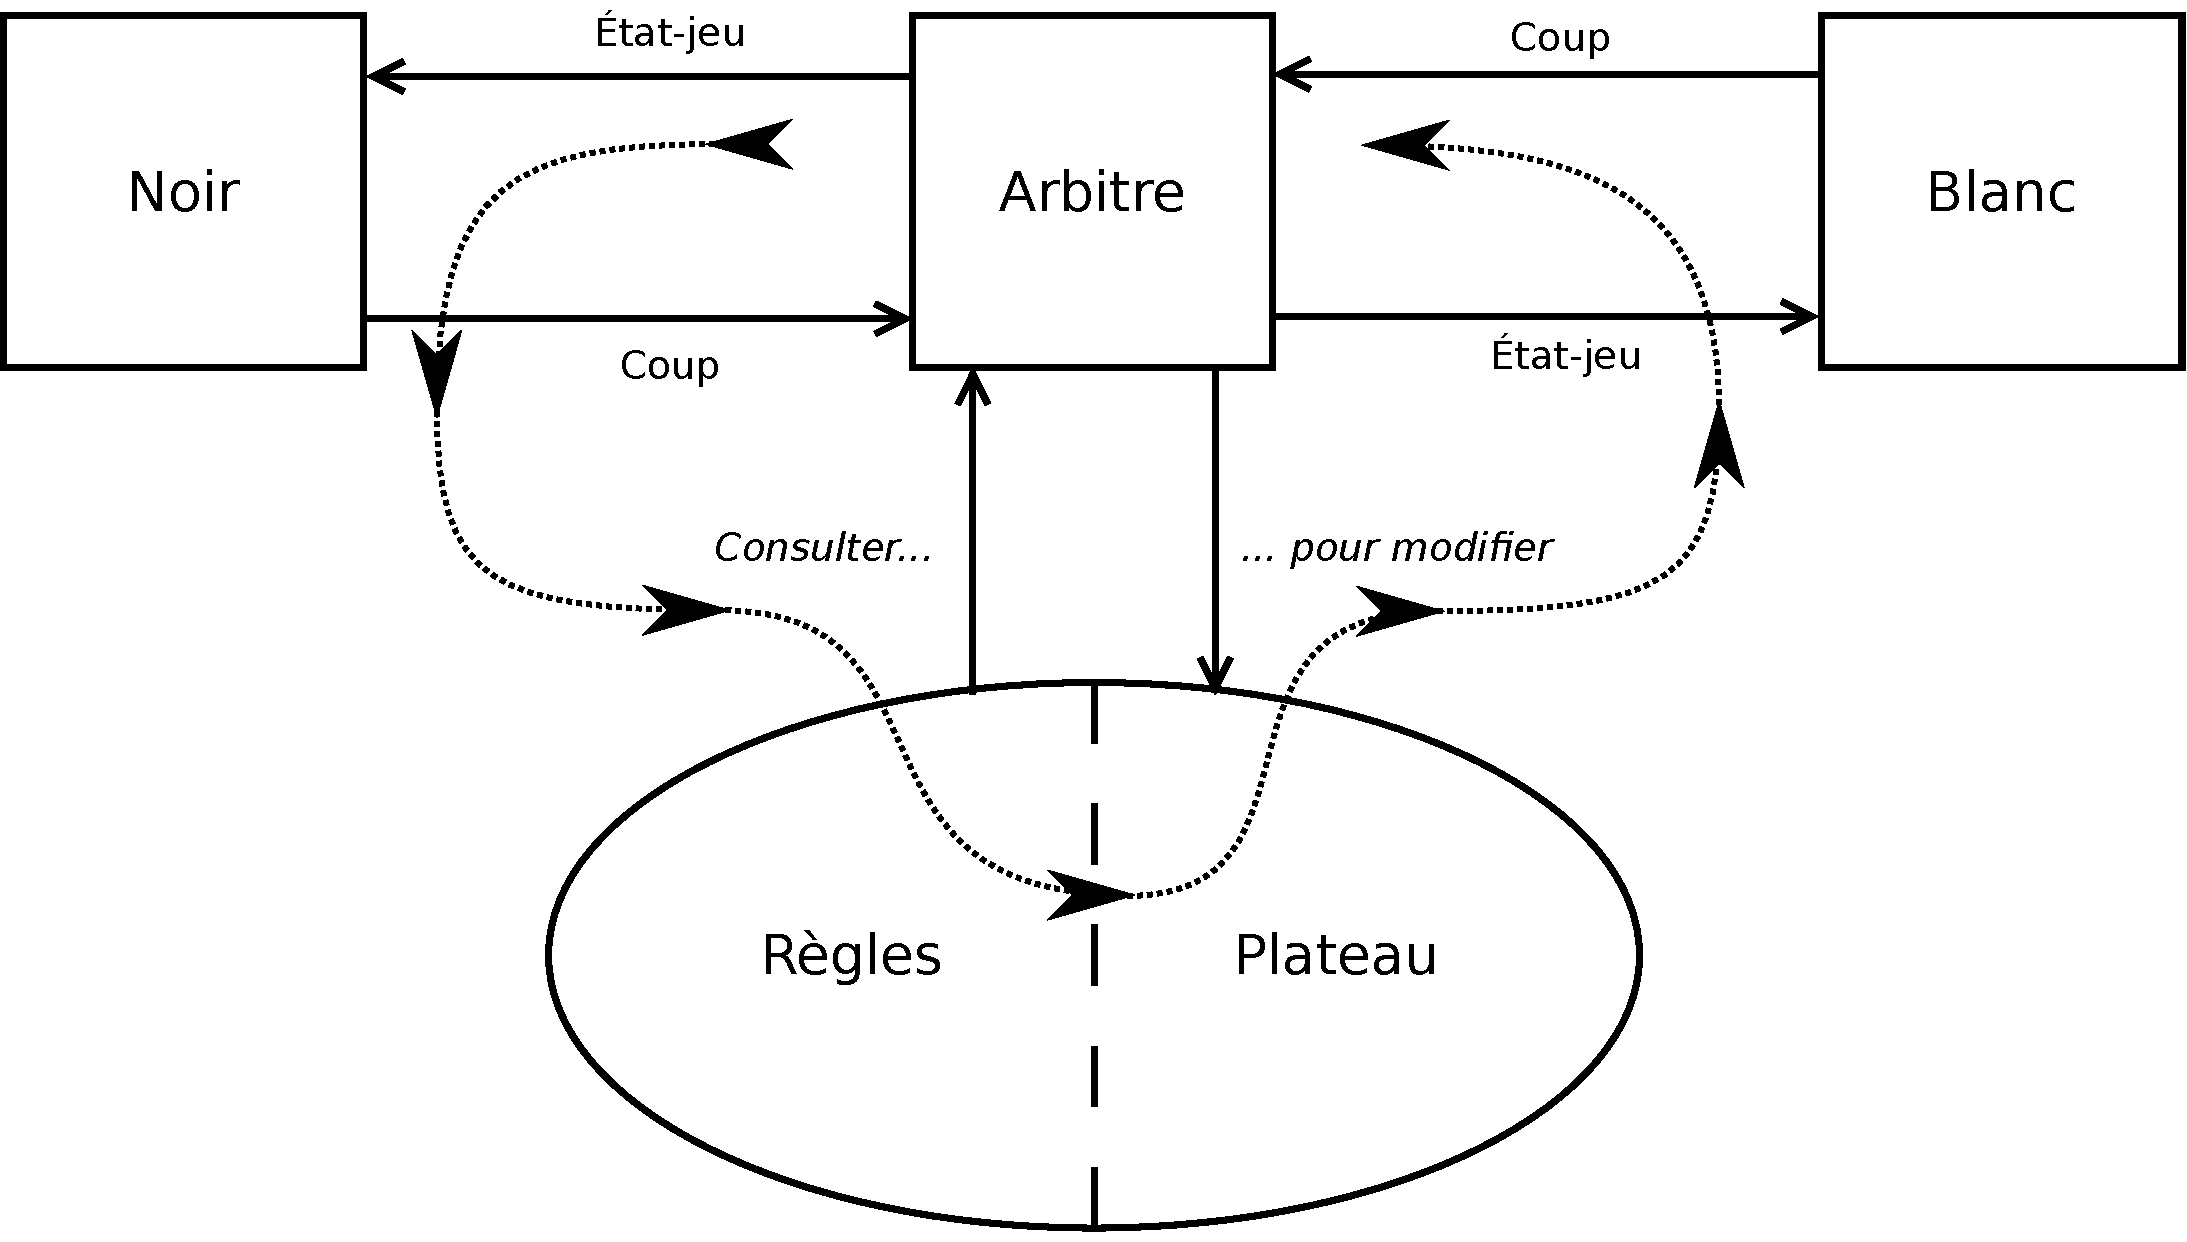
\includegraphics[width=\textwidth]{files/env/arbitre} 
\caption{Interactions entre l'Arbitre et les autres agents} 
\label{arbitre}
\end{figure}

C'est donc à travers cet \emph{agent-filtre} que les joueurs peuvent modifier l'environnement et, par conséquent, communiquer entre eux.

Suite à cette étude préalable, il est claire qu'une architecture \emph{client-serveur} est recommandé pour l'implémentation des interactions entre les agents et leur environnement.